% Based on the official DML course poster template.
\documentclass{beamer}
\usepackage[orientation=portrait,size=a2,scale=1.3]{beamerposter}
\mode<presentation>{\usetheme{ZH}}
\usepackage[utf8]{inputenc}
\usepackage[english]{babel}
\usepackage{helvet}
\usepackage{graphicx}
\usepackage{ragged2e}
\usepackage[font=scriptsize,justification=justified]{caption}
\usepackage{array,booktabs,tabularx}
\usepackage{amsmath}
\usepackage{tikz}
\usetikzlibrary{arrows.meta,positioning}

\newcolumntype{Z}{>{\centering\arraybackslash}X}
\title{Few-Shot Visual Adaptation of a Pretrained ViZDoom Agent}
\author{Paddington Xuchen Zhu \quad\textbullet\quad Ivan Sanchez}
\institute[Chalmers]{Chalmers University of Technology\\Deep Machine Learning}
\date{\today}

\newlength{\columnheight}
\setlength{\columnheight}{50cm}

\begin{document}
\begin{frame}
\begin{columns}
  \begin{column}{.48\textwidth}
    \begin{beamercolorbox}[center]{postercolumn}
      \begin{minipage}{.98\textwidth}
      \parbox[t][\columnheight]{\textwidth}{

      \begin{myblock}{Motivation and Research Question}
      A pretrained CNN+GRU agent performs well in the original ViZDoom Deadly Corridor, but visual domain shifts can sharply reduce completion. We ask:
      \begin{center}
      \textbf{Can the agent adapt to low light from only a few observations without retraining its policy?}
      \end{center}
      We reduce image brightness to $0.85$ and adapt with matched clean/dark observations. Performance is measured on unseen episode seeds using completion rate.

      \begin{figure}
      \centering
      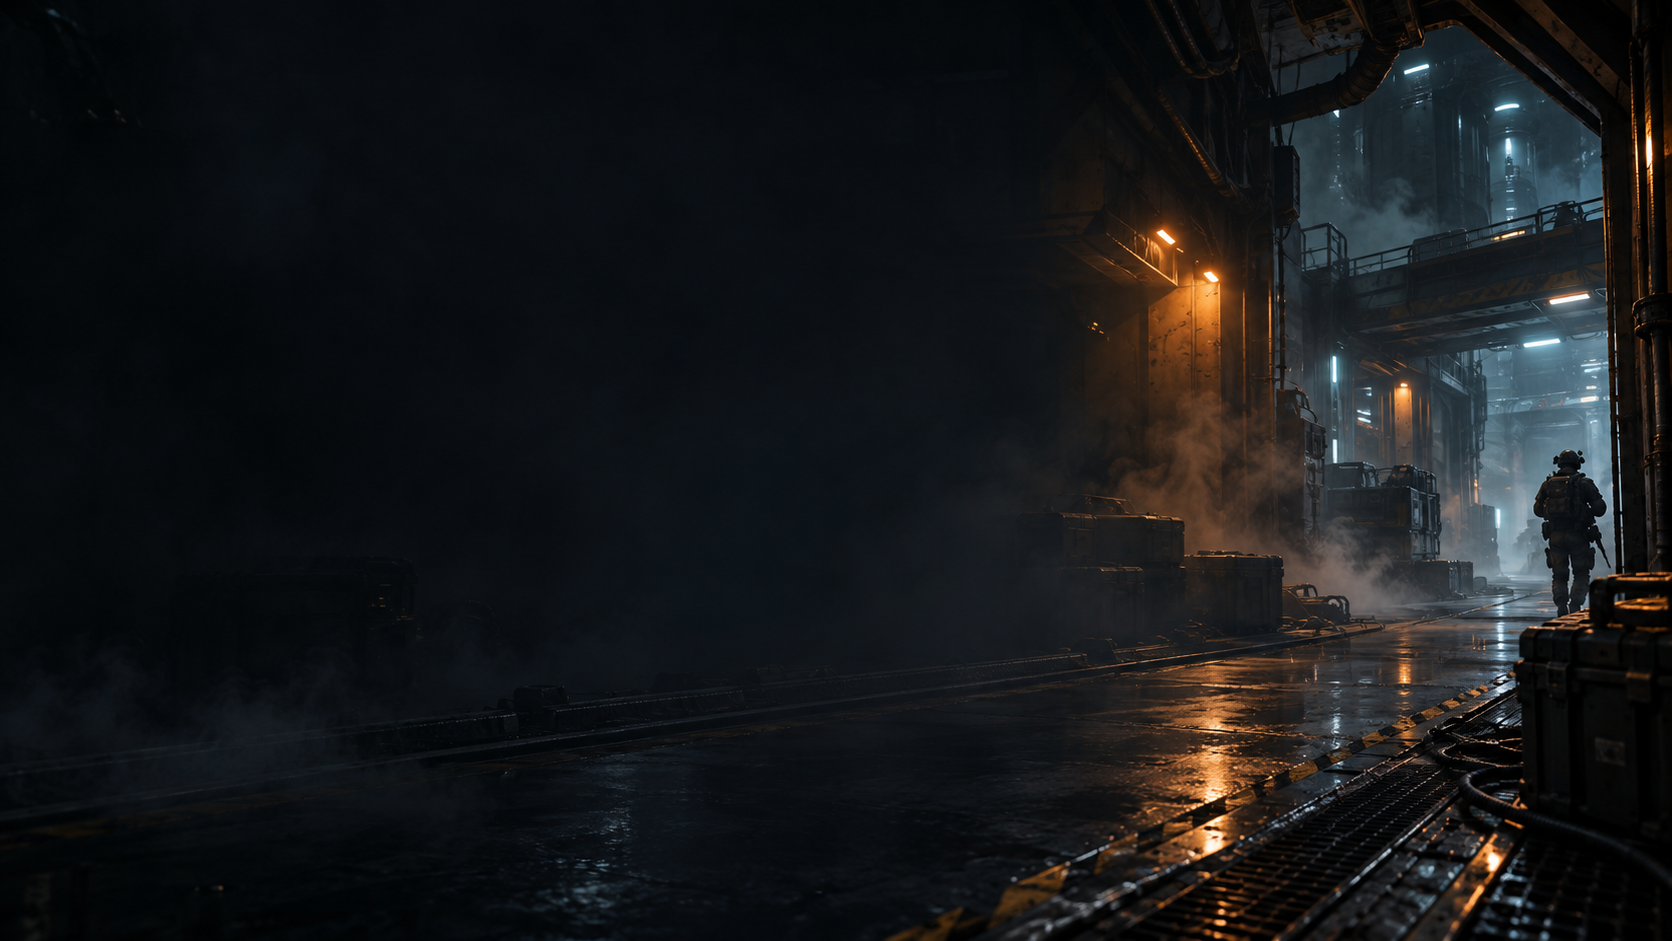
\includegraphics[width=.94\linewidth,height=7.0cm,keepaspectratio]{img/fps_corridor_background.png}
      \caption{A Call-of-Duty-style FPS context motivates robust perception under lighting shifts; experiments use ViZDoom Deadly Corridor.}
      \end{figure}
      \end{myblock}\vfill

      \begin{myblock}{Frozen-Policy Adapter Architecture}
      \centering
      \begin{tikzpicture}[node distance=0.55cm,>=Latex, every node/.style={font=\small}]
        \tikzstyle{frozen}=[draw=ETH8,very thick,rounded corners,minimum width=4.6cm,minimum height=1.5cm,fill=ETH8!8,align=center]
        \tikzstyle{trainable}=[draw=ETH3,very thick,rounded corners,minimum width=4.8cm,minimum height=1.5cm,fill=ETH3!10,align=center]
        \node[frozen] (rgb) {Low-light RGB\\$128\times72\times3$};
        \node[frozen,right=of rgb] (cnn) {Frozen CNN\\512 features};
        \node[trainable,right=of cnn] (adapter) {Trainable adapter\\6 or 8,712 parameters};
        \node[frozen,below=0.8cm of adapter] (gru) {Frozen GRU\\512 hidden units};
        \node[frozen,left=of gru] (heads) {Frozen heads\\action + value};
        \draw[->,very thick] (rgb)--(cnn);
        \draw[->,very thick] (cnn)--(adapter);
        \draw[->,very thick] (adapter)--(gru);
        \draw[->,very thick] (gru)--(heads);
      \end{tikzpicture}

      \vspace{0.5cm}
      The post-CNN residual bottleneck is identity-initialized:
      \[
      h' = h + W_{\mathrm{up}}\,\sigma(W_{\mathrm{down}}h).
      \]
      All 22 original Hugging Face policy tensors remain bit-identical. Only the adapter learns from policy-logit and value consistency.
      \end{myblock}\vfill

      \begin{myblock}{Controlled Experiments}
      \begin{enumerate}
        \item \textbf{Placement:} six parameters before CNN vs. after CNN.
        \item \textbf{Capacity:} six-parameter grouped affine vs. 8,712-parameter residual bottleneck.
        \item \textbf{Data budget:} 128, 512, 1,024, or 2,048 observations (512--8,192 game frames).
        \item \textbf{Baselines:} frozen upstream and full CNN+GRU fine-tuning.
        \item \textbf{Confirmation:} frozen best checkpoint, 500 fresh low-light and 500 fresh clean episodes per policy.
      \end{enumerate}
      Three independent adaptation seeds are used throughout, with matched evaluation seeds and paired outcomes.
      \end{myblock}\vfill

      \begin{myblock}{Parameter-Matched Placement}
      \begin{table}
      \centering
      \begin{tabularx}{\linewidth}{lZZZ}
      \toprule
      \textbf{Six-parameter adapter} & \textbf{Low-light mean} & \textbf{Worst seed} & \textbf{Clean mean}\\
      \midrule
      Before CNN (RGB) & 58.67\% & 58\% & --\\
      After CNN (features) & \textbf{68.00\%} & \textbf{67\%} & \textbf{84.33\%}\\
      Frozen upstream & -- & -- & 86.00\%\\
      \bottomrule
      \end{tabularx}
      \end{table}
      At equal capacity and equal 8,192-frame budget, post-CNN placement won all three matched comparisons and lost only 1.67 clean points.
      \end{myblock}

      }\end{minipage}
    \end{beamercolorbox}
  \end{column}

  \begin{column}{.52\textwidth}
    \begin{beamercolorbox}[center]{postercolumn}
      \begin{minipage}{.98\textwidth}
      \parbox[t][\columnheight]{\textwidth}{

      \begin{myblock}{Few-Shot Budget Curve}
        \begin{figure}
        \centering
        \begin{tikzpicture}[x=2.8cm,y=0.20cm,font=\scriptsize]
          \draw[->] (0,65) -- (4.55,65) node[right]{game frames};
          \draw[->] (0,65) -- (0,94) node[above]{completion (\%)};
          \foreach \y in {70,80,90}{\draw[gray!35] (0,\y)--(4.35,\y) node[left,black]{\y};}
          \foreach \x/\lab in {1/512,2/2,048,3/4,096,4/8,192}{\draw (\x,64.6)--(\x,65.4) node[below=4pt]{\lab};}
          \draw[ETH8,very thick] plot coordinates {(1,86) (2,88) (3,89) (4,89.67)};
          \foreach \x/\y in {1/86,2/88,3/89,4/89.67}{\fill[ETH8] (\x,\y) circle (3pt);}
          \draw[ETH3,very thick] plot coordinates {(1,74) (2,84) (3,87) (4,88)};
          \foreach \x/\y in {1/74,2/84,3/87,4/88}{\fill[ETH3] (\x,\y) rectangle +(5pt,5pt);}
          \draw[gray,very thick,dashed] plot coordinates {(1,71) (2,71) (3,71) (4,71)};
          \draw[ETH8,very thick] (0.35,92.5)--(.75,92.5) node[right,black]{8,712-param post-CNN};
          \draw[ETH3,very thick] (2.05,92.5)--(2.45,92.5) node[right,black]{6-param post-CNN};
          \draw[gray,very thick,dashed] (3.45,92.5)--(3.85,92.5) node[right,black]{upstream};
        \end{tikzpicture}
        \caption{Low-light completion on 100 unseen episodes per policy. The larger post-CNN adapter reaches 86\% after only 512 game frames.}
        \end{figure}
        Full CNN+GRU fine-tuning could not realize fewer than 8,192 frames and scored 68\% there, below its frozen baseline (69\%).
      \end{myblock}\vfill

      \begin{myblock}{Final 500-Episode Confirmation}
        \begin{figure}
        \centering
        \begin{tikzpicture}[x=2.2cm,y=0.10cm,font=\scriptsize]
          \draw[->] (0,50)--(4.4,50);
          \draw[->] (0,50)--(0,96) node[above]{completion (\%)};
          \foreach \y in {60,70,80,90}{\draw[gray!30] (0,\y)--(4.15,\y) node[left,black]{\y};}
          \fill[gray] (.65,50) rectangle (1.25,62.8);
          \fill[ETH8] (1.30,50) rectangle (1.90,78.27);
          \fill[gray] (2.65,50) rectangle (3.25,88.6);
          \fill[ETH8] (3.30,50) rectangle (3.90,79.47);
          \node[above] at (.95,62.8) {62.8};
          \node[above] at (1.60,78.27) {78.27};
          \node[above] at (2.95,88.6) {88.6};
          \node[above] at (3.60,79.47) {79.47};
          \node[below=5pt] at (1.28,50) {Low light};
          \node[below=5pt] at (3.28,50) {Clean};
          \fill[gray] (.8,93) rectangle +(0.25,2) node[right=5pt,black]{Frozen upstream};
          \fill[ETH8] (2.55,93) rectangle +(0.25,2) node[right=5pt,black]{Adapter mean};
        \end{tikzpicture}
        \caption{Mean completion across three independently adapted checkpoints on fresh, disjoint episode seeds.}
        \end{figure}
        \begin{columns}
          \begin{column}{.48\textwidth}
          \centering
          \textbf{Low light: confirmed}\par
          Upstream: 62.8\%\par
          Adapter: \textbf{78.27\%}\par
          \textbf{+15.47 points}
          \end{column}
          \begin{column}{.48\textwidth}
          \centering
          \textbf{Clean retention: failed}\par
          Upstream: 88.6\%\par
          Adapter: \textbf{79.47\%}\par
          \textbf{$-9.13$ points}
          \end{column}
        \end{columns}
        \vspace{0.5cm}
        All three adapter seeds won their paired low-light comparison. Candidate-only versus upstream-only successes were 96:11, 91:10, and 89:23.
      \end{myblock}\vfill

      \begin{myblock}{What Worked---and What Did Not}
      \begin{itemize}
        \item \textbf{Strong specialist:} 128 observations (512 frames) were sufficient for a reproducible low-light gain.
        \item \textbf{Safe small adapter:} the six-parameter post-CNN adapter reached 74\% low-light and 88\% clean at 512 frames.
        \item \textbf{Capacity tradeoff:} 8,712 parameters adapted faster, but exceeded the predefined five-point clean-retention limit.
        \item \textbf{Full fine-tuning was inefficient:} its smallest update required $16\times$ more frames and did not improve low-light completion.
        \item \textbf{Zero-shot generalization remained unsolved:} multi-domain GRU and GRU+attention training scored only 3.33\% and 2.8\% on the sealed combined shift.
      \end{itemize}
      \end{myblock}\vfill

      \begin{myblock}{Conclusion}
      \begin{center}
      \Large\textbf{A frozen post-CNN adapter can specialize a recurrent ViZDoom policy to low light with only 512 game frames.}
      \end{center}
      The 8,712-parameter adapter is best deployed as a \textbf{low-light specialist} behind a shift detector. The six-parameter post-CNN adapter is the safer always-on option because it improves low-light performance while preserving the clean domain.

      \vspace{0.5cm}
      \textbf{Next step:} learn a conditional gate that activates the specialist only under detected visual shift, combining high adaptation gain with clean-domain retention.
      \end{myblock}\vfill

      \begin{myblock}{Reproducibility}
      ViZDoom Deadly Corridor; pretrained Hugging Face CNN+GRU; brightness $0.85$; three adaptation seeds; disjoint matched test seeds; frozen-policy hash audits; no tuning on confirmation seeds.
      \end{myblock}

      }\end{minipage}
    \end{beamercolorbox}
  \end{column}
\end{columns}
\end{frame}
\end{document}
